\documentclass[../vis.tex]{subfiles}
\begin{document}
Beyond the basic panning and zooming, further interactions with the sky map are carried out in three directions:
the ability to easily and interactively query the catalog from the MongoDB database, the ability to filter the objects in the map based on their properties, and the ability to apply different colormaps to the displayed objects.
\textit{Vizic} utilizes advanced web technologies, such as HTML5 and D3.js\footnote{https://d3js.org} \citep{d3}, as well as the framework provided by \texttt{ipywidget}\footnote{https://github.com/ipython/ipywidgets} to make such interactivity possible.
\subsubsection{Data Query}
\label{data query}
\textit{Vizic} provides two methods to interactively query the catalog data. The first method is carried out through the selection tool and the query button widget. The selection tool allows users to make lasso-like selections on a sky map, where the geospatial coordinates of the selection bound are automatically stored in the \texttt{AstroMap} object.
When the query button is clicked, \textit{Vizic} sends a request to the database, asking for all of the objects that resides within the selection bounding box. The MongoDB engine retrieves the requested objects using the geospatial index and returns them to the IPython kernel where \textit{Vizic} then reads the returned data using a \textit{pandas} DataFrame and assign that DataFrame to the \texttt{select\_data} attribute of the corresponding \texttt{GridLayer} object.

The second method is to directly click on the displayed astronomical sources. Since these objects are drawn using Scalable Vector Graphics (SVG) elements instead of a HTML canvas, each object can individually responds to mouse events.
When such a SVG element catches a ``click'' event, it queries the database for the particular object it represents.
The returned data is first parsed into a \textit{pandas} Series object and then assigned to the \texttt{object\_catalog} attribute of the \texttt{GridLayer} object.
To continuously observe the data returned while clicking through different objects, a user can create a \texttt{PopupVis} widget for the rendered \texttt{GridLayer} widget. The \texttt{PopupVis} widget displays the data in a HTML table and constantly checks for updates from the \texttt{object\_catalog} attribute.

The selection tool mentioned and the \texttt{PopupVis} widget can be found in Figure \ref{fig:overall}, which shows a customized GUI built using the widgets provided by \textit{Vizic}.
Once data is retrieved from the MongoDB, it can be further processed from other notebook cells, providing a continuous analysis framework.

\subsubsection{Data Filter}
\label{filter}
\begin{figure}[h]
\centering
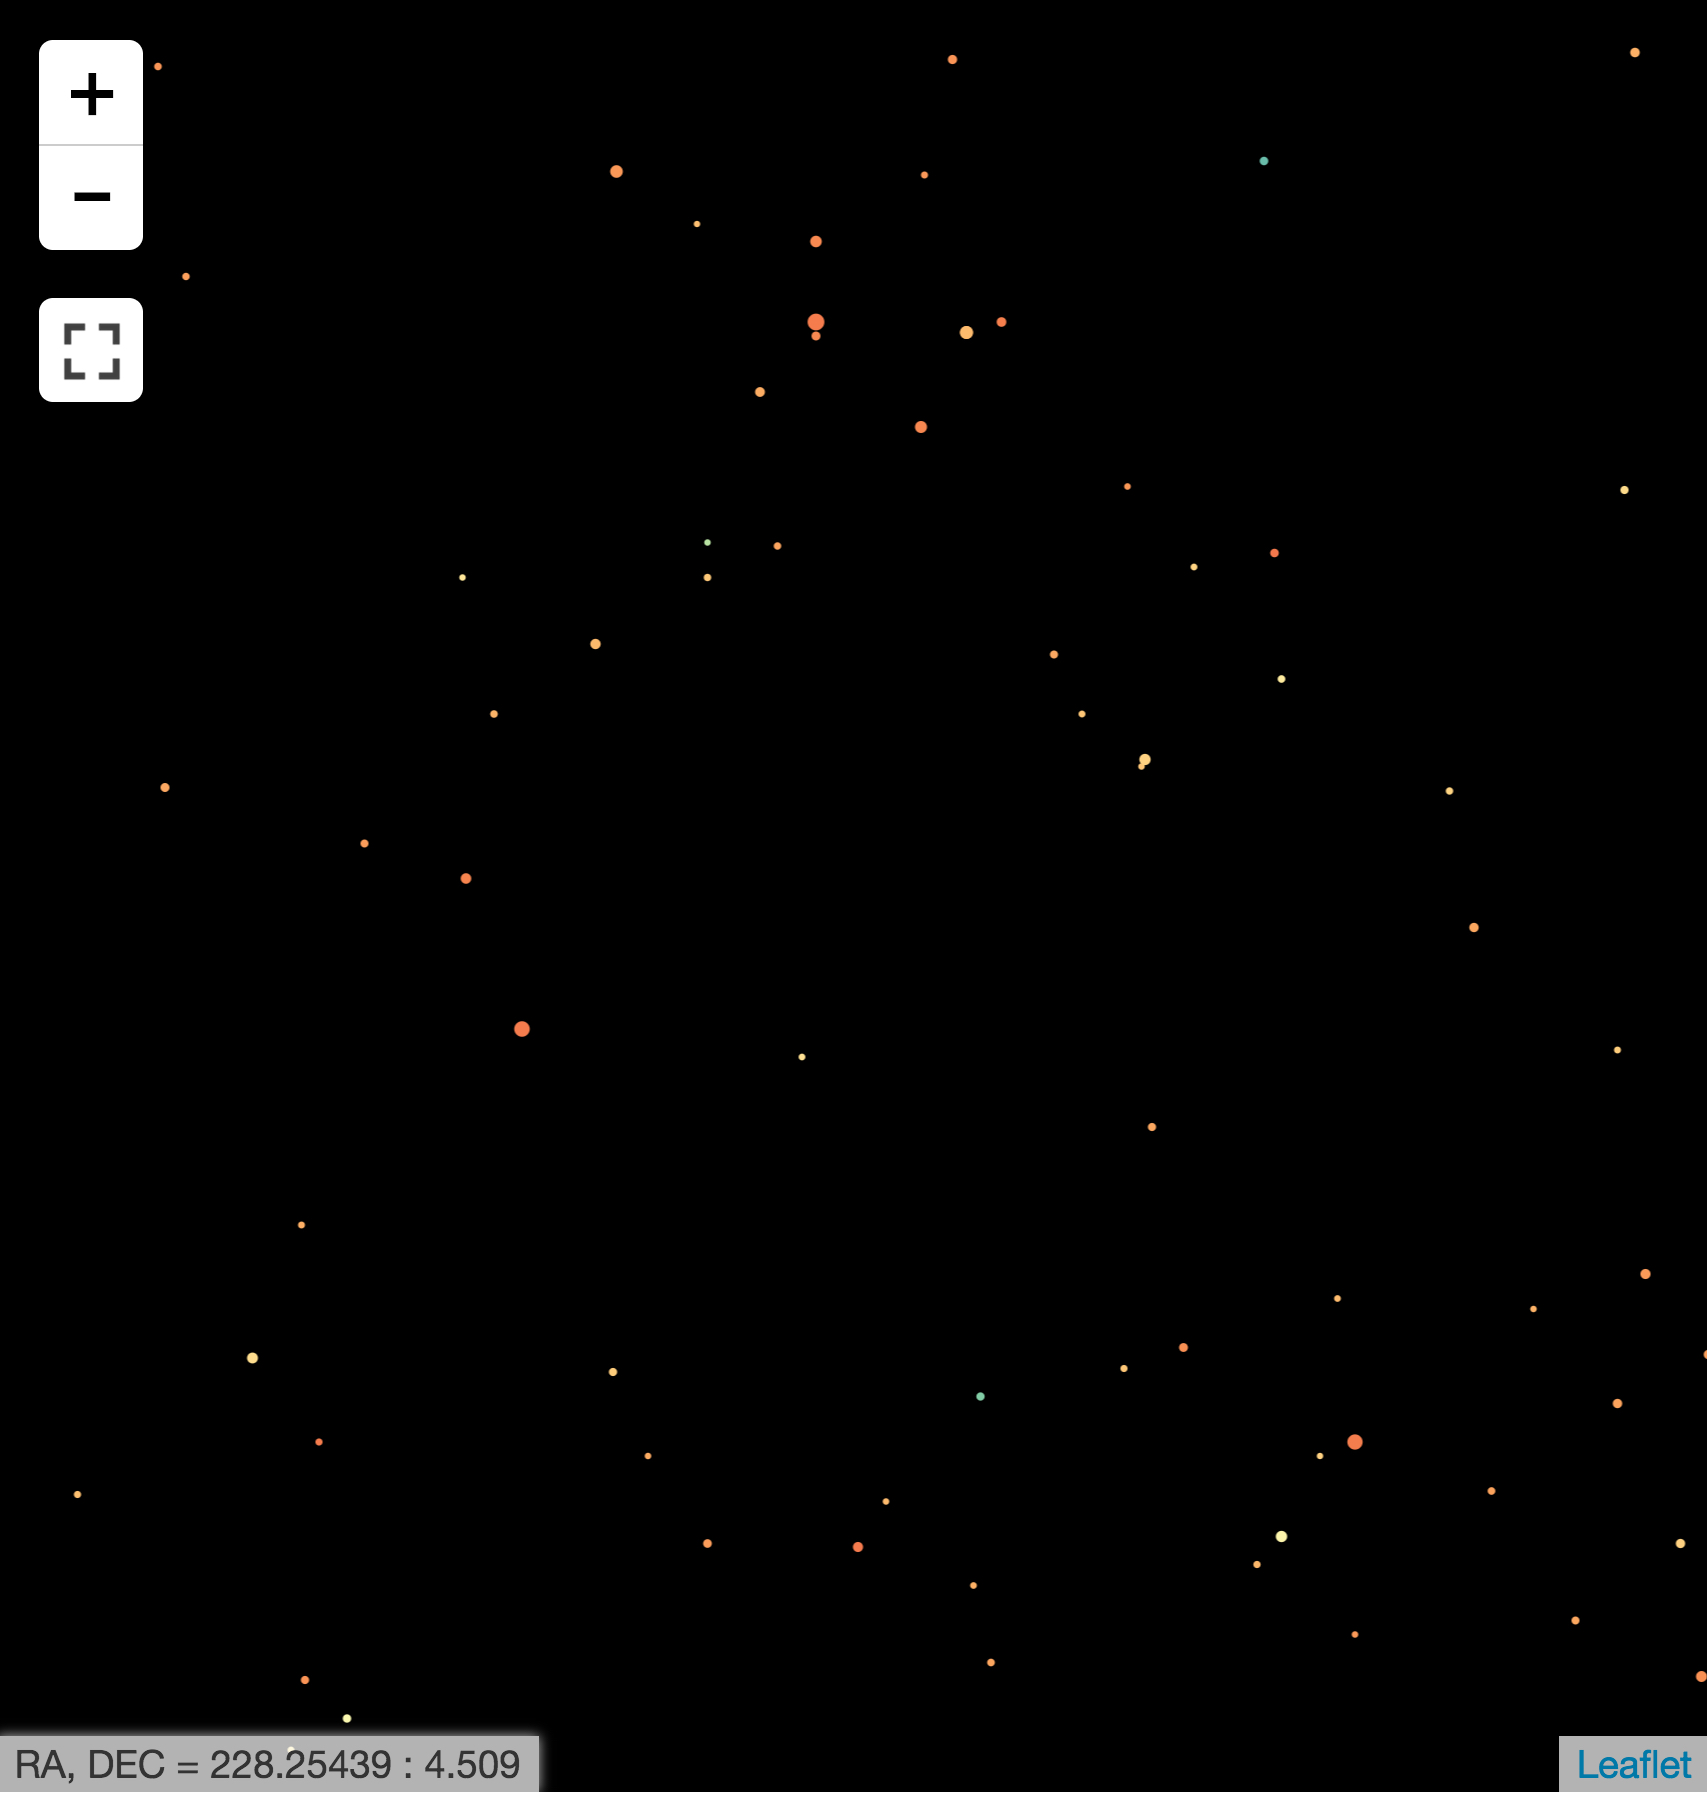
\includegraphics[width=0.43\textwidth]{FIG3}
\caption{The same area as shown in Figure \ref{fig:overall}, but only with object that has an $I$ magnitude \citep{sdss_filter} between $17.955$ and $27.249$.}
\label{fig:filtered}
\end{figure}
\textit{Vizic} also allows the users to filter displayed objects by their properties. In Jupyter notebooks, the filtering is controlled by a range slider bar.
The slider bar and another dropdown menu are wrapped into a single control widget, \texttt{FilterWidget}.
The dropdown menu in this control widget is responsible for switching the property field used to filter the objects. If a new property field is selected from the dropdown menu, the slider bar will updates itself with the new maximum value and minimum value for that particular field.
The property fields used to filter the object as well as the maximum and minimum values for each field are automatically determined and stored into the meta document\footnote{A document with `\_id' equals `meta'} in the catalog collection during the data ingestion process.

Every time the selected range on the slider bar changes, the \texttt{GridLayer} object validates the new range, updates the record and pushes the change to the front-end. As soon as the front-end widget receive the updates, it uses D3.js to select all objects that are outside the specified range and hides them. If a new property field is selected, \textit{Vizic} resets the filtering parameters and revalidates each object.

The objects filtering feature can be beneficial in many scenarios. For instance, we can easily determine outliers in the catalog by observing changes on the sky map while moving the slider bar from one side to another.
If the redshifts are provided, we can also visually inspect how cosmic structure evolves by shifting the selected range on the slide bar.
In Figure \ref{fig:filtered}, we shows the same area of the sky displayed by Figure \ref{fig:overall}, but only displaying the objects with an $I$ band magnitude between $17.955$ and $27.249$. Figure \ref{fig:slider} is a screenshot of the \texttt{FilterWidget} used.

\begin{figure}[h]
\centering
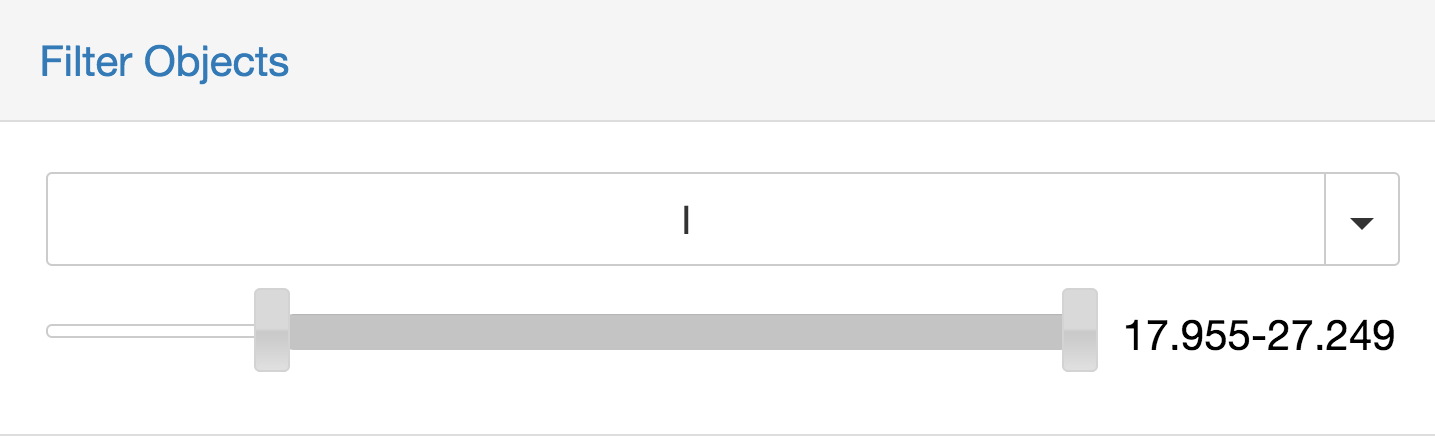
\includegraphics[width=0.45\textwidth]{FIG4}
\caption{A screenshot showing the FilterWidget}
\label{fig:slider}
\end{figure}
\subsubsection{Color Maps}
\label{color maps}
Color mapping is another powerful feature offered by \textit{Vizic} for visual inspections of a given dataset. The default colormap used by \textit{Vizic} is the spectral scheme. Any of the property field available in the filtering widget could be selected for color mapping. The \texttt{CFDropdown} control widget is a dropdown menu (see Figure \ref{fig:cdrop}) that serves as an interface for switching the property field used for color mapping.
When the custom color mapping mode is enabled, the front-end JavaScript maps the value of the selected property from each object in the catalog to a range of $[0, 1]$ in a continuous and linear scale. Using the scaled value, \textit{Vizic} selects the matching color from the colormap and assigns the color value to the SVG element representing the particular object.
\begin{figure}
\centering
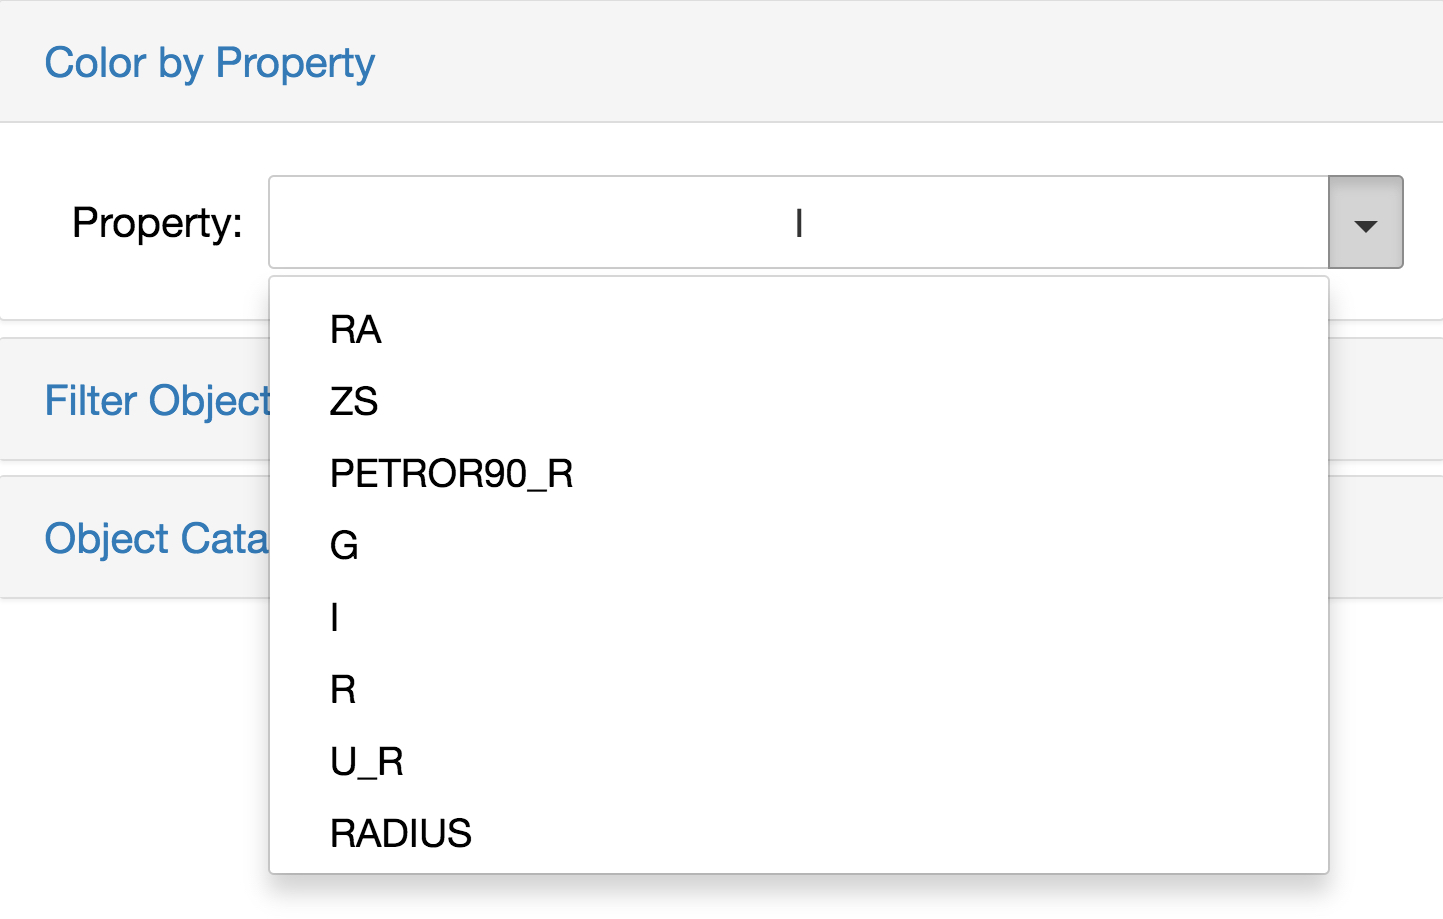
\includegraphics[width=0.45\textwidth]{FIG5}
\caption{A dropdown menu example showing properties that can be used for applying colormaps}
\label{fig:cdrop}
\end{figure}
Beside the spectral scheme, \textit{Vizic} provides a variety of additional colormaps defined in D3.js\footnote{https://github.com/d3/d3-scale-chromatic}. The user can change the colormap applied using the control widget, \texttt{ColorMap}. As a new colormap is chosen, the colors for the SVG elements will be reassigned based on the new color space. However, if the property field being used is changed, the scaled value of each object is subject to recalculation.

\end{document}
